\documentclass[10pt,journal]{IEEEtran}\usepackage{longtable}
\usepackage{graphicx} 
\usepackage{sidecap}
\usepackage{balance}
\usepackage{amsmath}
%\usepackage{cite}
\usepackage{amssymb}
\usepackage{amssymb}
\newcommand*{\QEDA}{\hfill\ensuremath{\blacksquare}}%
\newcommand*{\QEDB}{\hfill\ensuremath{\square}}%
\usepackage{siunitx}
\usepackage[none]{hyphenat}
\usepackage[margin=0.7in]{geometry}
\usepackage{esvect}
\usepackage{braket}
\usepackage{listings}
\usepackage{epstopdf}
\usepackage{subfigure}
\usepackage{color} %red, green, blue, yellow, cyan, magenta, black, white
\usepackage{verbatim}
\usepackage{mwe}
\usepackage{array}
\newcolumntype{$}{>{\global\let\currentrowstyle\relax}}
\newcolumntype{^}{>{\currentrowstyle}}
\newcommand{\rowstyle}[1]{\gdef\currentrowstyle{#1}%
  #1\ignorespaces
}
\usepackage{hhline}
\definecolor{mygreen}{RGB}{28,172,0} % color values Red, Green, Blue
\definecolor{mylilas}{RGB}{170,55,241}
\graphicspath{{Figures/}}
\DeclareSIUnit\uvrms{\micro\volt{}_{RMS}}
\DeclareSIUnit\mvrms{\milli\volt{}_{RMS}}

\begin{document}
\lstset{language=Matlab,%
    %basicstyle=\color{red},
    breaklines=true,%
    morekeywords={matlab2tikz},
    keywordstyle=\color{blue},%
    morekeywords=[2]{1}, keywordstyle=[2]{\color{black}},
    identifierstyle=\color{black},%
    stringstyle=\color{mylilas},
    commentstyle=\color{mygreen},%
    showstringspaces=false,%without this there will be a symbol in the places where there is a space
    numbers=left,%
    numberstyle={\tiny \color{black}},% size of the numbers
    numbersep=9pt, % this defines how far the numbers are from the text
    emph=[1]{for,end,break},emphstyle=[1]\color{red}, %some words to emphasise
    %emph=[2]{word1,word2}, emphstyle=[2]{style},    
}




%%%%%%%%%%%%%%%%%%%%%%%%%%%%%%%%%%%%%%%%%%%%%%%%%%%%%%%%%%%%%%%%%%%%%%%%%%%%%%%%%%%%%%%%%%
\title{EE 315\\Final Project}
\author{Thomas Flores and Samuel Lenius}
\date{\today}
\maketitle
%%%%%%%%%%%%%%%%%%%%%%%%%%%%%%%%%%%%%%%%%%%%%%%%%%%%%%%%%%%%%%%%%%%%%%%%%%%%%%%%%%%%%%%%%%

%%%%%% ABSTRACT %%%%%%%
\begin{abstract}
\lipsum[1]
\end{abstract}
%%%%%%%%%%%%%%%%%%%%%


%%%%%%% INTRODUCTION %%%%%%%%%%
\section{Introduction}
\lipsum[1-3]
%%%%%%%%%%%%%%%%%%%%%%%%%%%%

%%%%%%% COMPARATOR DESIGN %%%%%%%%%%%%
\section{Comparator}
\begin{figure}[tb]
\begin{center}
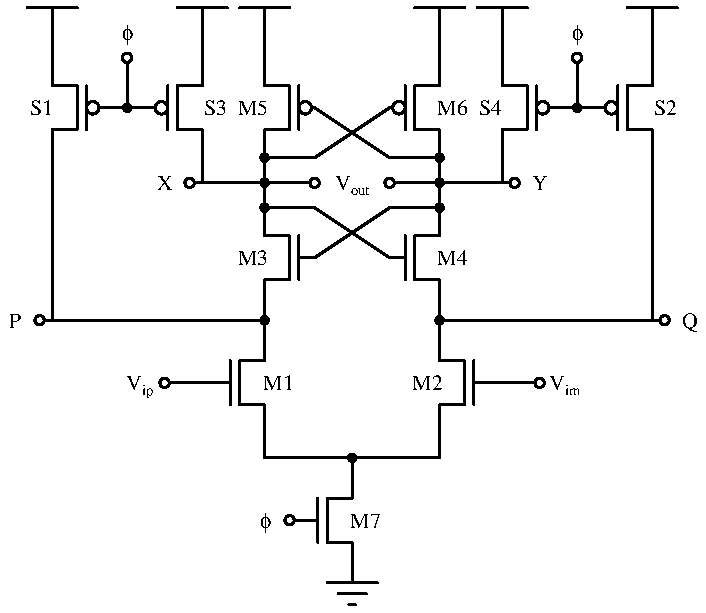
\includegraphics[width=1\columnwidth]{StrongArmLatch.pdf}
\caption{Circuit topology for the strong arm latch comparator.}
\label{fig:StrongArmLatch}
\end{center}
\end{figure}
Proper optimization of the comparator element in the SAR ADC will provide the greatest improvement in our figure of merit, as it will ultimately set the maximum speed of our design. Given that our figure of merit is proportional to the power consumed for each decision, the ideal design includes a dynamic comparator which only draws current during the decision time. For this reason, we choose the Strong Arm Latch \cite{Razavi:bp} for its energy efficiency and simple design.

To size our comparator to first order, we begin by considering the required noise specification of the total SAR ADC. We can derive the maximum noise power for our full-scale signal power as
\begin{equation}
\sigma_{n,in}^2=\frac{P_{sig}}{10^{SNR_{spec}/10}}=\frac{\frac{\left(0.5V_{FS}\right)^2}{2}}{10^{\frac{SNR_{spec}}{10}}}
\end{equation}
Because we are designing to first order and expect some noise contribution from the other blocks, we impose a slightly higher noise spec of \SI{60}{\decibel}. This gives an input referred noise requirement of $\sigma_{n,in}=\SI{707.11}{\uvrms}$ for $V_{FS}=\SI{2}{\volt}$.

We approximate the input referred noise for the strong arm latch as
\begin{equation}
\sigma_{n,in}^2\approx\frac{8\gamma}{A_v}\frac{kT}{C_{P,Q}}
\label{eq:InputNoise}
\end{equation}
where the gain $A_v$ during the amplification phase can be approximated as
\begin{equation}
A_v\approx\frac{g_{m1,2}}{I_D}V_{tn}
\label{eq:StrongArmGain}
\end{equation}
We select $\frac{g_m}{I_D}=15$ as this provides a reasonable tradeoff between speed and power of the transistor (SHOW CURVE?). From simulations, we find that the approximate threshold voltage $V_{tn}\approx\SI{250}{\milli\volt}$ for our nmos devices. We can then solve for the minimum capacitance necessary nodes P and Q using Equations \ref{eq:InputNoise}, \ref{eq:StrongArmGain}, and $\sigma_{n,in}=\SI{707}{\uvrms}$ 
\begin{equation}
C_{P,Q}\geq\frac{8\gamma}{A_v}\frac{kT}{\sigma_{n,in}^2}\rightarrow C_{P,Q}\geq\SI{14.79}{\femto\farad}
\end{equation}
To begin our design, we create a unit comparator constructed from some reasonable design choices. To maximize speed in the cross coupled inverters, we assume that pmos elements M5,6 should be twice the width of the nmos elements M3,4. To size M3,4, we must limit the widths so they do not signficantly contribute to the mismatch at the input. For our design with $A_v\approx3.5$, this means that $W3,4\geq\frac{1}{3.5}W1,2$ due to the offset referral to the input. 

\begin{table}[h]
\caption{Widths for comparators. All lengths minimum length $L=\SI{90}{\nano\metre}$}
\begin{center}
\begin{tabular}{c|c|c|c}
\hline \rowstyle{\bfseries} Transistor & \rowstyle{\bfseries} Unit & \rowstyle{\bfseries} First Order Design & \rowstyle{\bfseries} Optimized \\ \hline
M1,2 & \SI{1}{\micro\metre} & ? & ? \\ \hline
M3,4 & $\alpha W_{M1,2}$ & ? & ? \\ \hline
M5,6 & $2W_{M3,4}$ & ? & ? \\ \hline
M7 & ? & ? & ? \\ \hline
S1,2 & ? & ? & ? \\ \hline
S3,4 & ? & ? & ? \\ \hline
\end{tabular}
\end{center}
\label{tbl:ComparatorDesign}
\end{table}

%%%%%%%%%%%%%%%%%%%%%%%%%%%%%%%%%%


%%%%%%% BOOTSTRAPPED SWITCH DESIGN %%%%%%%%%%%%
\section{Track and Hold}
\begin{figure}[tbph]
\begin{center}
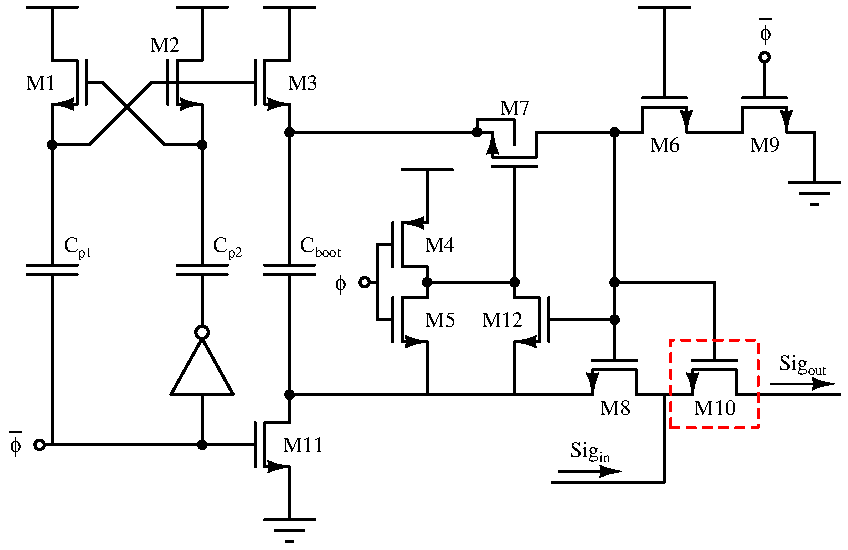
\includegraphics[width=1\columnwidth]{BootstrappedSwitch.pdf}
\caption{Circuit topology for the bootstrapped switch for improved linearity.}
\label{fig:BootstrappedSwitch}
\end{center}
\end{figure}
\lipsum[1-4]
%%%%%%%%%%%%%%%%%%%%%%%%%%%%%%%%%%


\bibliographystyle{IEEEtran}
\bibliography{IEEEabrv,References}
\end{document}


